In  diesem  Versuch kommen  verschiedene  Bereiche  aus der  Physik  zusammen,
prim\"ar Fluid-Dynamik und Optik. Entsprechend ergibt sich auch die Gliederung
dieses Kapitels.

% ---------------------------------------------------------------------------- %
\subsection{Messprinzip}
\label{subsec:messprinzip}
% ---------------------------------------------------------------------------- %

Das Verfahren nutzt den optischen  Dopplereffekt, um die Geschwindigkeit eines
Teilchens in einem  Fluid zu detektieren. Trifft ein  Lichtstrahl der Frequenz
$f$ auf  ein bewegtes Objekt,  unterschheidet sich die vom  Objekt detektierte
Frequenz $f_1$ ein wenig von der vom Sender emittierten Frequenz $f_0$.

\begin{equation}
    \label{eq:doppler}
    f_1 = f_0 \cdot \left( 1 - \frac{\vec{e} \cdot \vec{v}}{c} \right)
        = f_0 \cdot \left( 1 + \frac{v}{c} \cdot \cos{\vartheta_1} \right)
\end{equation}

Wobei $c$  die Lichtgeschwindigkeit, $\vec{e}$ ein  Einheitsvektor in Richtung
des  Lichtstrahls  und  $\vec{v}$   der  Geschwindigkeitsvektor  des  bewegten
Objektes ist. Wird der Lichtstrahl am bewegten Objekt gestreut und anschliessend
von einem Empf\"anger detektiert, ergibt sich f\"ur diesen die Frequenz $f_2$:

\begin{equation}
    \label{eq:doppler:gestreut}
    f_2
        = f_1 \cdot \left( 1 + \frac{\vec{a} \cdot \vec{v}}{c} \right)
        = f_0 \cdot \left( 1 - \frac{\vec{e} \cdot \vec{v}}{c} \right)
              \cdot \left( 1 + \frac{\vec{a} \cdot \vec{v}}{c} \right)
        \approx
        f_0 \cdot
        \left(
            1
            -
            \frac{\vec{a} \cdot \vec{v}}{c}
            +
            \frac{\vec{e} \cdot \vec{v}}{c}
        \right)
\end{equation}

$\vec{a}$   ist    dabei   ein   Einheitsvektor   in    Ausfallsrichtung   des
gestreuten   Strahls. Die   Konfiguration   ist   schematisch   in   Abbildung
\ref{fig:dopplereffekt} dargestellt.

\begin{figure}[h!t]
    \centering
    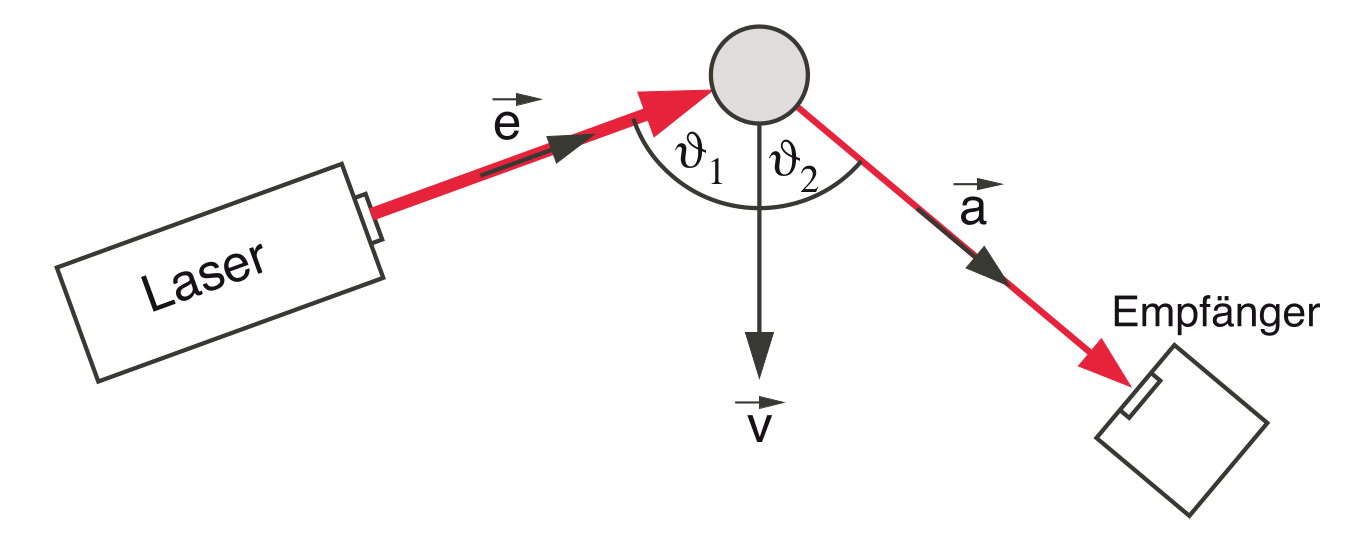
\includegraphics[width=0.67\textwidth]{images/doppler-effekt.png}
    \caption{%
        Dopplereffekt   mit  station\"arem   Sender,   bewegtem  Streuer   und
        station\"arem Detektor. \quelleVA
    }
    \label{fig:dopplereffekt}
\end{figure}

Da  bei  technischen  Geschwindigkeiten das  Verh\"altnis  $\frac{v}{c}$  sehr
klein   ist,  ergeben   sich  unter   solchen  Umst\"anden   lediglich  minime
Unterschide  in   den  Frequenzen  $f_4$,  $f_1$   und  $f_2$. Eine  pr\"azise
Messung  der  Frequenzunterschiede  ist  somit enorm  schwierig,  weshalb  man
sich  eines Zwei-Stral-Verfahrens  bedient. Da die  beiden Teilstrahlen  dabei
in  unterschiedlichen  Winkeln  $\vartheta_1$  (vgl. Formel  \ref{eq:doppler})
auf   das   streuende   Teilchen  treffen,   erfahren   sie   unterschiedliche
Doppler-Verschiebungen ihrer Frequenzen.

\"Uberlagert man  nun die beiden  Teilstrahlen in einem Detektor,  ergibt sich
eine  Schwebung, deren  Frequenz bedeutend  tiefer  als $f_0$  ist, und  somit
verh\"altnism\"assig gut detektiert werden kann.

Eine     h\"aufig     verwendete     Konfiguration    ist     in     Abbildung
\ref{fig:zweistrahl-anordnung} zu sehen.

\begin{figure}[h!t]
    \centering
    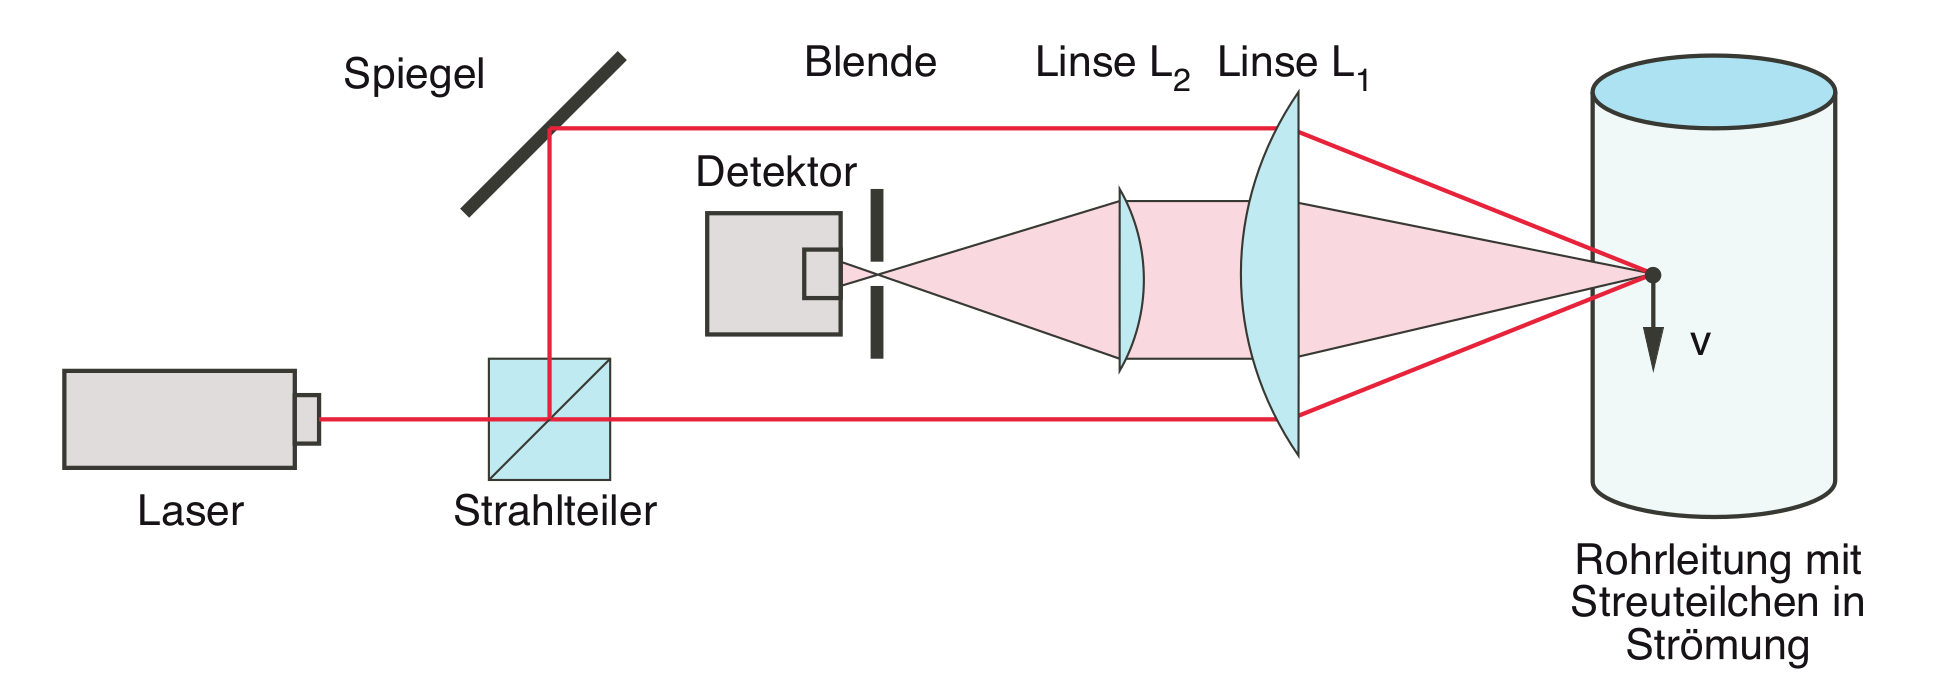
\includegraphics[width=0.67\textwidth]{images/zweistrahl-anordnung.png}
    \caption{%
        Zwei-Srahl-Anordnung. \quelleVA
    }
    \label{fig:zweistrahl-anordnung}
\end{figure}

Ein Strahlteiler teilt  den Laserstrahl auf zwei Strahlen auf  und ein Spiegel
sorgt daf\"ur, dass zwei parallele  Strahlen entstehen, die anschliessen durch
eine Linse $L_1$ mit Brennweite $f_1$ wieder zusammengef\"uhrt werden. Fliesst
ein Streuteilchen durch diesen Schnittpunkt, ergeben sich f\"ur die beiden Teilstrahlen
zwei unterschiedliche Frequenzen aufgrund des Dopplereffekts:

\begin{align}
    \label{eq:splitFreqs1}
        f_1 &= f_0 \cdot
            \left(
                1 + \frac{v}{c} \cdot \cos\left( \SI{90}{\degree} + \frac{\varphi}{2} \right)
            \right)
            =
            f_0 \cdot
            \left(
                1 - \frac{v}{c} \cdot \sin\left(\frac{\varphi}{2}\right)
            \right)
            \\
        \label{eq:splitFreqs2}
        f_2 &= f_0 \cdot
            \left(
                1 + \frac{v}{c} \cdot \cos\left( \SI{90}{\degree} - \frac{\varphi}{2} \right)
            \right)
            =
            f_0 \cdot
            \left(
                1 + \frac{v}{c} \cdot \sin\left(\frac{\varphi}{2}\right)
            \right)
            \\
        \label{eq:splitFreqsDelta}
        \Delta f &= f_2 - f_1 = f_0 \cdot \frac{2 \cdot v}{c} \cdot \sin\left( \frac{\varphi}{2}\right)
\end{align}

Die beiden  Wellenz\"uge werden  anschliessend in einem  einzelnen Empf\"anger
zusammengef\"uhrt. Die durch diese \"Uberlagerung erzeugte Schwebung errechnet
sich  nach  einigen  trigonometrischen  Umformungen zu  (beachte,  dass  beide
Signale die gleiche Amplitude haben, was die Sache etwas vereinfacht):

\begin{equation}
    \label{eq:schwebung}
    S(t) = A \cdot \cos(\omega_1 \cdot t) + A \cdot \cos(\omega_2 \cdot t)
         = 2 A \cdot
             \cos\left(
                 \frac{\omega_1 + \omega_2}{2} \cdot t
             \right)
             \cdot
             \cos\left(
                 \frac{\omega_1 - \omega_2}{2} \cdot t
             \right)
\end{equation}

% ---------------------------------------------------------------------------- %
\clearpage
\subsection{Grundlagen aus der Fluid-Dynamik}
\label{subsec:fluiddynamik}
% ---------------------------------------------------------------------------- %

\subsubsection{Vorbereitung auf Messaufgaben}

3.1 -- Zusammenhang zwischen maximaler und durchschnittlicher Str\"omungsgeschwindigkeit im laminaren Fall

\textbf{fix: avg over flaeche}
\begin{equation}
    \label{eq:laminar:v_max:v_avg}
    \frac{v(r)}{v_{max}} = \frac{1}{v_{max} \cdot R} \cdot \int_0^R\!v(r) \, \mathrm{d}r
    = \frac{1}{R} \cdot \int_0^R \! 1 - \frac{r^2}{R^2} \, \mathrm{d}r
    = \frac{1}{2}
\end{equation}

3.2 -- Zusammenhang zwischen maximaler und durchschnittlicher Str\"omungsgeschwindigkeit im turbulenten Fall:

\begin{align}
    \label{eq:turbulent:v_max:v_avg}
    v(r) &= v_{max} \cdot \left( 1 - \frac{r}{R} \right) ^ \frac{1}{k}
    \\
    v_m &= \frac{1}{\pi \cdot R^2} \cdot \int_0^R \! v(r) \cdot 2 \cdot \pi \cdot r \, \mathrm{d}r
    \\
    \frac{v_m}{v_{max}} &= \frac{2}{R^2} \cdot \int_0^R \! \left(1 - \frac{r}{R} \right) ^ \frac{1}{k} \cdot r \, \mathrm{d}r = \frac{2 \cdot k^2}{(k + 1) \cdot (2k + 1)}
\end{align}

3.3 -- Vergleich von laminarem und turbulentem Str\"omungsprofil

%\begin{figure}[h!t]
%    \centering
%    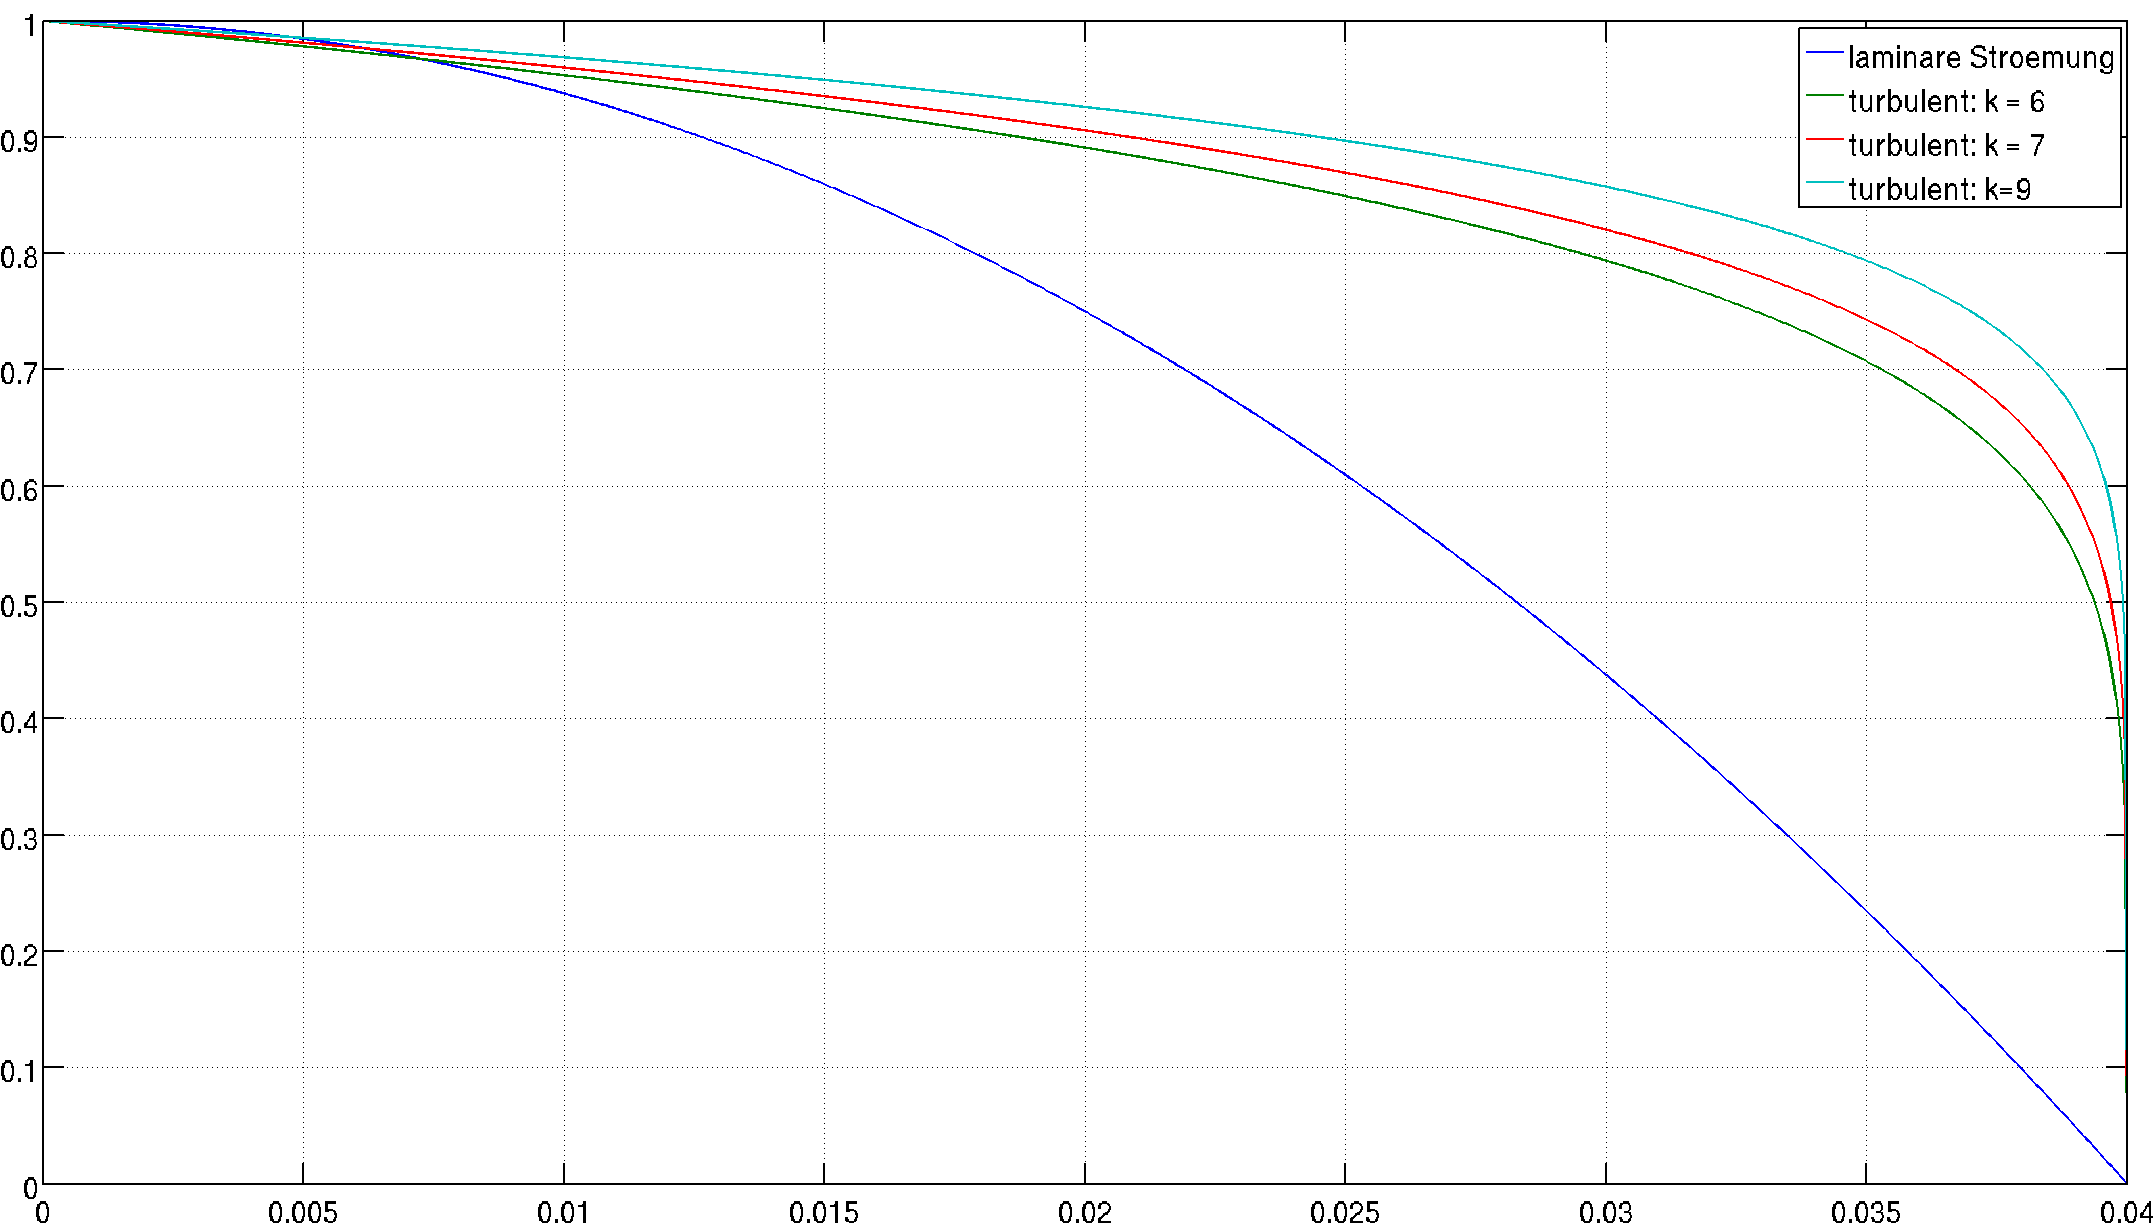
\includegraphics[width=\textwidth]{images/laminar-vs-turbulent.png}
%    \caption{%
%        Laminares vs. turbulente Str\"omungsprofile
%    }
%    \label{fig:dopplereffekt}
%\end{figure}

\begin{figure}[h!t]
    \centering
    \resizebox{.9\textwidth}{!}{%% Creator: Matplotlib, PGF backend
%%
%% To include the figure in your LaTeX document, write
%%   \input{<filename>.pgf}
%%
%% Make sure the required packages are loaded in your preamble
%%   \usepackage{pgf}
%%
%% Figures using additional raster images can only be included by \input if
%% they are in the same directory as the main LaTeX file. For loading figures
%% from other directories you can use the `import` package
%%   \usepackage{import}
%% and then include the figures with
%%   \import{<path to file>}{<filename>.pgf}
%%
%% Matplotlib used the following preamble
%%   \usepackage{fontspec}
%%   \setmainfont{Bitstream Vera Serif}
%%   \setsansfont{Bitstream Vera Sans}
%%   \setmonofont{Bitstream Vera Sans Mono}
%%
\begingroup%
\makeatletter%
\begin{pgfpicture}%
\pgfpathrectangle{\pgfpointorigin}{\pgfqpoint{8.000000in}{6.000000in}}%
\pgfusepath{use as bounding box, clip}%
\begin{pgfscope}%
\pgfsetbuttcap%
\pgfsetmiterjoin%
\definecolor{currentfill}{rgb}{1.000000,1.000000,1.000000}%
\pgfsetfillcolor{currentfill}%
\pgfsetlinewidth{0.000000pt}%
\definecolor{currentstroke}{rgb}{1.000000,1.000000,1.000000}%
\pgfsetstrokecolor{currentstroke}%
\pgfsetdash{}{0pt}%
\pgfpathmoveto{\pgfqpoint{0.000000in}{0.000000in}}%
\pgfpathlineto{\pgfqpoint{8.000000in}{0.000000in}}%
\pgfpathlineto{\pgfqpoint{8.000000in}{6.000000in}}%
\pgfpathlineto{\pgfqpoint{0.000000in}{6.000000in}}%
\pgfpathclose%
\pgfusepath{fill}%
\end{pgfscope}%
\begin{pgfscope}%
\pgfsetbuttcap%
\pgfsetmiterjoin%
\definecolor{currentfill}{rgb}{1.000000,1.000000,1.000000}%
\pgfsetfillcolor{currentfill}%
\pgfsetlinewidth{0.000000pt}%
\definecolor{currentstroke}{rgb}{0.000000,0.000000,0.000000}%
\pgfsetstrokecolor{currentstroke}%
\pgfsetstrokeopacity{0.000000}%
\pgfsetdash{}{0pt}%
\pgfpathmoveto{\pgfqpoint{1.000000in}{0.600000in}}%
\pgfpathlineto{\pgfqpoint{7.200000in}{0.600000in}}%
\pgfpathlineto{\pgfqpoint{7.200000in}{5.400000in}}%
\pgfpathlineto{\pgfqpoint{1.000000in}{5.400000in}}%
\pgfpathclose%
\pgfusepath{fill}%
\end{pgfscope}%
\begin{pgfscope}%
\pgfpathrectangle{\pgfqpoint{1.000000in}{0.600000in}}{\pgfqpoint{6.200000in}{4.800000in}} %
\pgfusepath{clip}%
\pgfsetrectcap%
\pgfsetroundjoin%
\pgfsetlinewidth{1.003750pt}%
\definecolor{currentstroke}{rgb}{0.000000,0.000000,1.000000}%
\pgfsetstrokecolor{currentstroke}%
\pgfsetdash{}{0pt}%
\pgfpathmoveto{\pgfqpoint{1.000000in}{5.400000in}}%
\pgfpathlineto{\pgfqpoint{1.091268in}{5.398918in}}%
\pgfpathlineto{\pgfqpoint{1.182535in}{5.395671in}}%
\pgfpathlineto{\pgfqpoint{1.273803in}{5.390261in}}%
\pgfpathlineto{\pgfqpoint{1.365071in}{5.382685in}}%
\pgfpathlineto{\pgfqpoint{1.456339in}{5.372946in}}%
\pgfpathlineto{\pgfqpoint{1.547606in}{5.361042in}}%
\pgfpathlineto{\pgfqpoint{1.638874in}{5.346974in}}%
\pgfpathlineto{\pgfqpoint{1.730142in}{5.330742in}}%
\pgfpathlineto{\pgfqpoint{1.821410in}{5.312345in}}%
\pgfpathlineto{\pgfqpoint{1.912677in}{5.291784in}}%
\pgfpathlineto{\pgfqpoint{2.003945in}{5.269058in}}%
\pgfpathlineto{\pgfqpoint{2.095213in}{5.244168in}}%
\pgfpathlineto{\pgfqpoint{2.192565in}{5.215234in}}%
\pgfpathlineto{\pgfqpoint{2.289917in}{5.183837in}}%
\pgfpathlineto{\pgfqpoint{2.387270in}{5.149977in}}%
\pgfpathlineto{\pgfqpoint{2.484622in}{5.113655in}}%
\pgfpathlineto{\pgfqpoint{2.581974in}{5.074870in}}%
\pgfpathlineto{\pgfqpoint{2.679326in}{5.033623in}}%
\pgfpathlineto{\pgfqpoint{2.776679in}{4.989913in}}%
\pgfpathlineto{\pgfqpoint{2.874031in}{4.943741in}}%
\pgfpathlineto{\pgfqpoint{2.971383in}{4.895106in}}%
\pgfpathlineto{\pgfqpoint{3.068735in}{4.844009in}}%
\pgfpathlineto{\pgfqpoint{3.166088in}{4.790449in}}%
\pgfpathlineto{\pgfqpoint{3.263440in}{4.734426in}}%
\pgfpathlineto{\pgfqpoint{3.360792in}{4.675941in}}%
\pgfpathlineto{\pgfqpoint{3.458144in}{4.614994in}}%
\pgfpathlineto{\pgfqpoint{3.561581in}{4.547539in}}%
\pgfpathlineto{\pgfqpoint{3.665018in}{4.477304in}}%
\pgfpathlineto{\pgfqpoint{3.768455in}{4.404290in}}%
\pgfpathlineto{\pgfqpoint{3.871891in}{4.328495in}}%
\pgfpathlineto{\pgfqpoint{3.975328in}{4.249920in}}%
\pgfpathlineto{\pgfqpoint{4.078765in}{4.168566in}}%
\pgfpathlineto{\pgfqpoint{4.182202in}{4.084431in}}%
\pgfpathlineto{\pgfqpoint{4.285639in}{3.997516in}}%
\pgfpathlineto{\pgfqpoint{4.389075in}{3.907822in}}%
\pgfpathlineto{\pgfqpoint{4.498597in}{3.809821in}}%
\pgfpathlineto{\pgfqpoint{4.608118in}{3.708704in}}%
\pgfpathlineto{\pgfqpoint{4.717639in}{3.604470in}}%
\pgfpathlineto{\pgfqpoint{4.827160in}{3.497119in}}%
\pgfpathlineto{\pgfqpoint{4.936682in}{3.386652in}}%
\pgfpathlineto{\pgfqpoint{5.046203in}{3.273068in}}%
\pgfpathlineto{\pgfqpoint{5.155724in}{3.156368in}}%
\pgfpathlineto{\pgfqpoint{5.265246in}{3.036551in}}%
\pgfpathlineto{\pgfqpoint{5.380851in}{2.906696in}}%
\pgfpathlineto{\pgfqpoint{5.496457in}{2.773369in}}%
\pgfpathlineto{\pgfqpoint{5.612063in}{2.636569in}}%
\pgfpathlineto{\pgfqpoint{5.727669in}{2.496296in}}%
\pgfpathlineto{\pgfqpoint{5.843275in}{2.352551in}}%
\pgfpathlineto{\pgfqpoint{5.958880in}{2.205334in}}%
\pgfpathlineto{\pgfqpoint{6.074486in}{2.054644in}}%
\pgfpathlineto{\pgfqpoint{6.196177in}{1.892271in}}%
\pgfpathlineto{\pgfqpoint{6.317867in}{1.726051in}}%
\pgfpathlineto{\pgfqpoint{6.439557in}{1.555983in}}%
\pgfpathlineto{\pgfqpoint{6.561248in}{1.382067in}}%
\pgfpathlineto{\pgfqpoint{6.682938in}{1.204304in}}%
\pgfpathlineto{\pgfqpoint{6.804628in}{1.022693in}}%
\pgfpathlineto{\pgfqpoint{6.926318in}{0.837234in}}%
\pgfpathlineto{\pgfqpoint{7.054093in}{0.638361in}}%
\pgfpathlineto{\pgfqpoint{7.078431in}{0.600000in}}%
\pgfpathlineto{\pgfqpoint{7.078431in}{0.600000in}}%
\pgfusepath{stroke}%
\end{pgfscope}%
\begin{pgfscope}%
\pgfpathrectangle{\pgfqpoint{1.000000in}{0.600000in}}{\pgfqpoint{6.200000in}{4.800000in}} %
\pgfusepath{clip}%
\pgfsetrectcap%
\pgfsetroundjoin%
\pgfsetlinewidth{1.003750pt}%
\definecolor{currentstroke}{rgb}{0.000000,0.500000,0.000000}%
\pgfsetstrokecolor{currentstroke}%
\pgfsetdash{}{0pt}%
\pgfpathmoveto{\pgfqpoint{1.000000in}{5.400000in}}%
\pgfpathlineto{\pgfqpoint{1.346817in}{5.353230in}}%
\pgfpathlineto{\pgfqpoint{1.675381in}{5.306692in}}%
\pgfpathlineto{\pgfqpoint{1.985692in}{5.260522in}}%
\pgfpathlineto{\pgfqpoint{2.277748in}{5.214874in}}%
\pgfpathlineto{\pgfqpoint{2.557636in}{5.168901in}}%
\pgfpathlineto{\pgfqpoint{2.819270in}{5.123730in}}%
\pgfpathlineto{\pgfqpoint{3.068735in}{5.078452in}}%
\pgfpathlineto{\pgfqpoint{3.306032in}{5.033148in}}%
\pgfpathlineto{\pgfqpoint{3.531159in}{4.987917in}}%
\pgfpathlineto{\pgfqpoint{3.744117in}{4.942873in}}%
\pgfpathlineto{\pgfqpoint{3.944906in}{4.898150in}}%
\pgfpathlineto{\pgfqpoint{4.133526in}{4.853906in}}%
\pgfpathlineto{\pgfqpoint{4.316061in}{4.808781in}}%
\pgfpathlineto{\pgfqpoint{4.486428in}{4.764363in}}%
\pgfpathlineto{\pgfqpoint{4.644625in}{4.720883in}}%
\pgfpathlineto{\pgfqpoint{4.796738in}{4.676795in}}%
\pgfpathlineto{\pgfqpoint{4.942766in}{4.632102in}}%
\pgfpathlineto{\pgfqpoint{5.076626in}{4.588837in}}%
\pgfpathlineto{\pgfqpoint{5.204400in}{4.545228in}}%
\pgfpathlineto{\pgfqpoint{5.326091in}{4.501327in}}%
\pgfpathlineto{\pgfqpoint{5.441697in}{4.457202in}}%
\pgfpathlineto{\pgfqpoint{5.551218in}{4.412934in}}%
\pgfpathlineto{\pgfqpoint{5.654655in}{4.368625in}}%
\pgfpathlineto{\pgfqpoint{5.752007in}{4.324401in}}%
\pgfpathlineto{\pgfqpoint{5.843275in}{4.280411in}}%
\pgfpathlineto{\pgfqpoint{5.928458in}{4.236838in}}%
\pgfpathlineto{\pgfqpoint{6.007557in}{4.193898in}}%
\pgfpathlineto{\pgfqpoint{6.080571in}{4.151847in}}%
\pgfpathlineto{\pgfqpoint{6.153585in}{4.107149in}}%
\pgfpathlineto{\pgfqpoint{6.220515in}{4.063513in}}%
\pgfpathlineto{\pgfqpoint{6.281360in}{4.021308in}}%
\pgfpathlineto{\pgfqpoint{6.342205in}{3.976327in}}%
\pgfpathlineto{\pgfqpoint{6.396966in}{3.933113in}}%
\pgfpathlineto{\pgfqpoint{6.451726in}{3.886900in}}%
\pgfpathlineto{\pgfqpoint{6.500402in}{3.842905in}}%
\pgfpathlineto{\pgfqpoint{6.549078in}{3.795706in}}%
\pgfpathlineto{\pgfqpoint{6.591670in}{3.751340in}}%
\pgfpathlineto{\pgfqpoint{6.634262in}{3.703612in}}%
\pgfpathlineto{\pgfqpoint{6.670769in}{3.659563in}}%
\pgfpathlineto{\pgfqpoint{6.707276in}{3.612095in}}%
\pgfpathlineto{\pgfqpoint{6.743783in}{3.560562in}}%
\pgfpathlineto{\pgfqpoint{6.774206in}{3.513905in}}%
\pgfpathlineto{\pgfqpoint{6.804628in}{3.463183in}}%
\pgfpathlineto{\pgfqpoint{6.835051in}{3.407525in}}%
\pgfpathlineto{\pgfqpoint{6.859389in}{3.358655in}}%
\pgfpathlineto{\pgfqpoint{6.883727in}{3.305029in}}%
\pgfpathlineto{\pgfqpoint{6.908065in}{3.245493in}}%
\pgfpathlineto{\pgfqpoint{6.926318in}{3.195994in}}%
\pgfpathlineto{\pgfqpoint{6.944572in}{3.141270in}}%
\pgfpathlineto{\pgfqpoint{6.962826in}{3.079929in}}%
\pgfpathlineto{\pgfqpoint{6.981079in}{3.009907in}}%
\pgfpathlineto{\pgfqpoint{6.999333in}{2.927935in}}%
\pgfpathlineto{\pgfqpoint{7.011502in}{2.864014in}}%
\pgfpathlineto{\pgfqpoint{7.023671in}{2.789546in}}%
\pgfpathlineto{\pgfqpoint{7.035840in}{2.699729in}}%
\pgfpathlineto{\pgfqpoint{7.048009in}{2.585220in}}%
\pgfpathlineto{\pgfqpoint{7.054093in}{2.512745in}}%
\pgfpathlineto{\pgfqpoint{7.060178in}{2.423198in}}%
\pgfpathlineto{\pgfqpoint{7.066262in}{2.304062in}}%
\pgfpathlineto{\pgfqpoint{7.072347in}{2.118146in}}%
\pgfpathlineto{\pgfqpoint{7.078431in}{0.600000in}}%
\pgfpathlineto{\pgfqpoint{7.078431in}{0.600000in}}%
\pgfusepath{stroke}%
\end{pgfscope}%
\begin{pgfscope}%
\pgfpathrectangle{\pgfqpoint{1.000000in}{0.600000in}}{\pgfqpoint{6.200000in}{4.800000in}} %
\pgfusepath{clip}%
\pgfsetrectcap%
\pgfsetroundjoin%
\pgfsetlinewidth{1.003750pt}%
\definecolor{currentstroke}{rgb}{1.000000,0.000000,0.000000}%
\pgfsetstrokecolor{currentstroke}%
\pgfsetdash{}{0pt}%
\pgfpathmoveto{\pgfqpoint{1.000000in}{5.400000in}}%
\pgfpathlineto{\pgfqpoint{1.365071in}{5.357715in}}%
\pgfpathlineto{\pgfqpoint{1.711888in}{5.315341in}}%
\pgfpathlineto{\pgfqpoint{2.040452in}{5.272974in}}%
\pgfpathlineto{\pgfqpoint{2.350763in}{5.230727in}}%
\pgfpathlineto{\pgfqpoint{2.642819in}{5.188735in}}%
\pgfpathlineto{\pgfqpoint{2.916623in}{5.147156in}}%
\pgfpathlineto{\pgfqpoint{3.178257in}{5.105174in}}%
\pgfpathlineto{\pgfqpoint{3.421637in}{5.063895in}}%
\pgfpathlineto{\pgfqpoint{3.652849in}{5.022437in}}%
\pgfpathlineto{\pgfqpoint{3.871891in}{4.980886in}}%
\pgfpathlineto{\pgfqpoint{4.078765in}{4.939346in}}%
\pgfpathlineto{\pgfqpoint{4.273470in}{4.897942in}}%
\pgfpathlineto{\pgfqpoint{4.456005in}{4.856825in}}%
\pgfpathlineto{\pgfqpoint{4.626371in}{4.816172in}}%
\pgfpathlineto{\pgfqpoint{4.784569in}{4.776194in}}%
\pgfpathlineto{\pgfqpoint{4.936682in}{4.735459in}}%
\pgfpathlineto{\pgfqpoint{5.076626in}{4.695730in}}%
\pgfpathlineto{\pgfqpoint{5.210485in}{4.655434in}}%
\pgfpathlineto{\pgfqpoint{5.338260in}{4.614591in}}%
\pgfpathlineto{\pgfqpoint{5.453866in}{4.575359in}}%
\pgfpathlineto{\pgfqpoint{5.563387in}{4.535918in}}%
\pgfpathlineto{\pgfqpoint{5.666824in}{4.496357in}}%
\pgfpathlineto{\pgfqpoint{5.764176in}{4.456784in}}%
\pgfpathlineto{\pgfqpoint{5.855444in}{4.417332in}}%
\pgfpathlineto{\pgfqpoint{5.940627in}{4.378163in}}%
\pgfpathlineto{\pgfqpoint{6.019726in}{4.339473in}}%
\pgfpathlineto{\pgfqpoint{6.098824in}{4.298220in}}%
\pgfpathlineto{\pgfqpoint{6.171839in}{4.257523in}}%
\pgfpathlineto{\pgfqpoint{6.238768in}{4.217670in}}%
\pgfpathlineto{\pgfqpoint{6.299613in}{4.179001in}}%
\pgfpathlineto{\pgfqpoint{6.360458in}{4.137651in}}%
\pgfpathlineto{\pgfqpoint{6.415219in}{4.097783in}}%
\pgfpathlineto{\pgfqpoint{6.469980in}{4.054985in}}%
\pgfpathlineto{\pgfqpoint{6.518656in}{4.014075in}}%
\pgfpathlineto{\pgfqpoint{6.567332in}{3.969992in}}%
\pgfpathlineto{\pgfqpoint{6.609924in}{3.928362in}}%
\pgfpathlineto{\pgfqpoint{6.652515in}{3.883351in}}%
\pgfpathlineto{\pgfqpoint{6.689022in}{3.841586in}}%
\pgfpathlineto{\pgfqpoint{6.725529in}{3.796319in}}%
\pgfpathlineto{\pgfqpoint{6.755952in}{3.755419in}}%
\pgfpathlineto{\pgfqpoint{6.786375in}{3.711066in}}%
\pgfpathlineto{\pgfqpoint{6.816797in}{3.662559in}}%
\pgfpathlineto{\pgfqpoint{6.841135in}{3.620138in}}%
\pgfpathlineto{\pgfqpoint{6.865473in}{3.573809in}}%
\pgfpathlineto{\pgfqpoint{6.889811in}{3.522695in}}%
\pgfpathlineto{\pgfqpoint{6.914149in}{3.465579in}}%
\pgfpathlineto{\pgfqpoint{6.932403in}{3.417766in}}%
\pgfpathlineto{\pgfqpoint{6.950657in}{3.364524in}}%
\pgfpathlineto{\pgfqpoint{6.968910in}{3.304310in}}%
\pgfpathlineto{\pgfqpoint{6.987164in}{3.234783in}}%
\pgfpathlineto{\pgfqpoint{6.999333in}{3.181467in}}%
\pgfpathlineto{\pgfqpoint{7.011502in}{3.120590in}}%
\pgfpathlineto{\pgfqpoint{7.023671in}{3.049358in}}%
\pgfpathlineto{\pgfqpoint{7.035840in}{2.962981in}}%
\pgfpathlineto{\pgfqpoint{7.048009in}{2.852085in}}%
\pgfpathlineto{\pgfqpoint{7.054093in}{2.781426in}}%
\pgfpathlineto{\pgfqpoint{7.060178in}{2.693592in}}%
\pgfpathlineto{\pgfqpoint{7.066262in}{2.575769in}}%
\pgfpathlineto{\pgfqpoint{7.072347in}{2.389501in}}%
\pgfpathlineto{\pgfqpoint{7.078431in}{0.600000in}}%
\pgfpathlineto{\pgfqpoint{7.078431in}{0.600000in}}%
\pgfusepath{stroke}%
\end{pgfscope}%
\begin{pgfscope}%
\pgfpathrectangle{\pgfqpoint{1.000000in}{0.600000in}}{\pgfqpoint{6.200000in}{4.800000in}} %
\pgfusepath{clip}%
\pgfsetrectcap%
\pgfsetroundjoin%
\pgfsetlinewidth{1.003750pt}%
\definecolor{currentstroke}{rgb}{0.000000,0.750000,0.750000}%
\pgfsetstrokecolor{currentstroke}%
\pgfsetdash{}{0pt}%
\pgfpathmoveto{\pgfqpoint{1.000000in}{5.400000in}}%
\pgfpathlineto{\pgfqpoint{1.407663in}{5.363117in}}%
\pgfpathlineto{\pgfqpoint{1.790987in}{5.326220in}}%
\pgfpathlineto{\pgfqpoint{2.149974in}{5.289442in}}%
\pgfpathlineto{\pgfqpoint{2.484622in}{5.252947in}}%
\pgfpathlineto{\pgfqpoint{2.794932in}{5.216928in}}%
\pgfpathlineto{\pgfqpoint{3.086989in}{5.180844in}}%
\pgfpathlineto{\pgfqpoint{3.360792in}{5.144816in}}%
\pgfpathlineto{\pgfqpoint{3.616342in}{5.108995in}}%
\pgfpathlineto{\pgfqpoint{3.853638in}{5.073562in}}%
\pgfpathlineto{\pgfqpoint{4.078765in}{5.037735in}}%
\pgfpathlineto{\pgfqpoint{4.291723in}{5.001573in}}%
\pgfpathlineto{\pgfqpoint{4.486428in}{4.966292in}}%
\pgfpathlineto{\pgfqpoint{4.668963in}{4.931008in}}%
\pgfpathlineto{\pgfqpoint{4.839330in}{4.895863in}}%
\pgfpathlineto{\pgfqpoint{4.997527in}{4.861030in}}%
\pgfpathlineto{\pgfqpoint{5.149640in}{4.825243in}}%
\pgfpathlineto{\pgfqpoint{5.289584in}{4.790029in}}%
\pgfpathlineto{\pgfqpoint{5.417359in}{4.755669in}}%
\pgfpathlineto{\pgfqpoint{5.539049in}{4.720686in}}%
\pgfpathlineto{\pgfqpoint{5.654655in}{4.685097in}}%
\pgfpathlineto{\pgfqpoint{5.758091in}{4.651005in}}%
\pgfpathlineto{\pgfqpoint{5.855444in}{4.616677in}}%
\pgfpathlineto{\pgfqpoint{5.946711in}{4.582211in}}%
\pgfpathlineto{\pgfqpoint{6.031895in}{4.547737in}}%
\pgfpathlineto{\pgfqpoint{6.110993in}{4.513415in}}%
\pgfpathlineto{\pgfqpoint{6.184008in}{4.479442in}}%
\pgfpathlineto{\pgfqpoint{6.250937in}{4.446060in}}%
\pgfpathlineto{\pgfqpoint{6.317867in}{4.410186in}}%
\pgfpathlineto{\pgfqpoint{6.378712in}{4.375049in}}%
\pgfpathlineto{\pgfqpoint{6.433473in}{4.341021in}}%
\pgfpathlineto{\pgfqpoint{6.488233in}{4.304321in}}%
\pgfpathlineto{\pgfqpoint{6.536909in}{4.269062in}}%
\pgfpathlineto{\pgfqpoint{6.585586in}{4.230865in}}%
\pgfpathlineto{\pgfqpoint{6.628177in}{4.194584in}}%
\pgfpathlineto{\pgfqpoint{6.670769in}{4.155113in}}%
\pgfpathlineto{\pgfqpoint{6.707276in}{4.118246in}}%
\pgfpathlineto{\pgfqpoint{6.743783in}{4.078002in}}%
\pgfpathlineto{\pgfqpoint{6.774206in}{4.041364in}}%
\pgfpathlineto{\pgfqpoint{6.804628in}{4.001312in}}%
\pgfpathlineto{\pgfqpoint{6.835051in}{3.957089in}}%
\pgfpathlineto{\pgfqpoint{6.859389in}{3.918018in}}%
\pgfpathlineto{\pgfqpoint{6.883727in}{3.874878in}}%
\pgfpathlineto{\pgfqpoint{6.908065in}{3.826647in}}%
\pgfpathlineto{\pgfqpoint{6.926318in}{3.786272in}}%
\pgfpathlineto{\pgfqpoint{6.944572in}{3.741335in}}%
\pgfpathlineto{\pgfqpoint{6.962826in}{3.690579in}}%
\pgfpathlineto{\pgfqpoint{6.981079in}{3.632126in}}%
\pgfpathlineto{\pgfqpoint{6.993248in}{3.587471in}}%
\pgfpathlineto{\pgfqpoint{7.005417in}{3.536738in}}%
\pgfpathlineto{\pgfqpoint{7.017586in}{3.477844in}}%
\pgfpathlineto{\pgfqpoint{7.029755in}{3.407369in}}%
\pgfpathlineto{\pgfqpoint{7.041924in}{3.319051in}}%
\pgfpathlineto{\pgfqpoint{7.048009in}{3.264523in}}%
\pgfpathlineto{\pgfqpoint{7.054093in}{3.199272in}}%
\pgfpathlineto{\pgfqpoint{7.060178in}{3.117501in}}%
\pgfpathlineto{\pgfqpoint{7.066262in}{3.006600in}}%
\pgfpathlineto{\pgfqpoint{7.072347in}{2.828210in}}%
\pgfpathlineto{\pgfqpoint{7.078431in}{0.600000in}}%
\pgfpathlineto{\pgfqpoint{7.078431in}{0.600000in}}%
\pgfusepath{stroke}%
\end{pgfscope}%
\begin{pgfscope}%
\pgfsetrectcap%
\pgfsetmiterjoin%
\pgfsetlinewidth{1.003750pt}%
\definecolor{currentstroke}{rgb}{0.000000,0.000000,0.000000}%
\pgfsetstrokecolor{currentstroke}%
\pgfsetdash{}{0pt}%
\pgfpathmoveto{\pgfqpoint{7.200000in}{0.600000in}}%
\pgfpathlineto{\pgfqpoint{7.200000in}{5.400000in}}%
\pgfusepath{stroke}%
\end{pgfscope}%
\begin{pgfscope}%
\pgfsetrectcap%
\pgfsetmiterjoin%
\pgfsetlinewidth{1.003750pt}%
\definecolor{currentstroke}{rgb}{0.000000,0.000000,0.000000}%
\pgfsetstrokecolor{currentstroke}%
\pgfsetdash{}{0pt}%
\pgfpathmoveto{\pgfqpoint{1.000000in}{0.600000in}}%
\pgfpathlineto{\pgfqpoint{1.000000in}{5.400000in}}%
\pgfusepath{stroke}%
\end{pgfscope}%
\begin{pgfscope}%
\pgfsetrectcap%
\pgfsetmiterjoin%
\pgfsetlinewidth{1.003750pt}%
\definecolor{currentstroke}{rgb}{0.000000,0.000000,0.000000}%
\pgfsetstrokecolor{currentstroke}%
\pgfsetdash{}{0pt}%
\pgfpathmoveto{\pgfqpoint{1.000000in}{5.400000in}}%
\pgfpathlineto{\pgfqpoint{7.200000in}{5.400000in}}%
\pgfusepath{stroke}%
\end{pgfscope}%
\begin{pgfscope}%
\pgfsetrectcap%
\pgfsetmiterjoin%
\pgfsetlinewidth{1.003750pt}%
\definecolor{currentstroke}{rgb}{0.000000,0.000000,0.000000}%
\pgfsetstrokecolor{currentstroke}%
\pgfsetdash{}{0pt}%
\pgfpathmoveto{\pgfqpoint{1.000000in}{0.600000in}}%
\pgfpathlineto{\pgfqpoint{7.200000in}{0.600000in}}%
\pgfusepath{stroke}%
\end{pgfscope}%
\begin{pgfscope}%
\pgfsetbuttcap%
\pgfsetroundjoin%
\definecolor{currentfill}{rgb}{0.000000,0.000000,0.000000}%
\pgfsetfillcolor{currentfill}%
\pgfsetlinewidth{0.501875pt}%
\definecolor{currentstroke}{rgb}{0.000000,0.000000,0.000000}%
\pgfsetstrokecolor{currentstroke}%
\pgfsetdash{}{0pt}%
\pgfsys@defobject{currentmarker}{\pgfqpoint{0.000000in}{0.000000in}}{\pgfqpoint{0.000000in}{0.055556in}}{%
\pgfpathmoveto{\pgfqpoint{0.000000in}{0.000000in}}%
\pgfpathlineto{\pgfqpoint{0.000000in}{0.055556in}}%
\pgfusepath{stroke,fill}%
}%
\begin{pgfscope}%
\pgfsys@transformshift{1.000000in}{0.600000in}%
\pgfsys@useobject{currentmarker}{}%
\end{pgfscope}%
\end{pgfscope}%
\begin{pgfscope}%
\pgfsetbuttcap%
\pgfsetroundjoin%
\definecolor{currentfill}{rgb}{0.000000,0.000000,0.000000}%
\pgfsetfillcolor{currentfill}%
\pgfsetlinewidth{0.501875pt}%
\definecolor{currentstroke}{rgb}{0.000000,0.000000,0.000000}%
\pgfsetstrokecolor{currentstroke}%
\pgfsetdash{}{0pt}%
\pgfsys@defobject{currentmarker}{\pgfqpoint{0.000000in}{-0.055556in}}{\pgfqpoint{0.000000in}{0.000000in}}{%
\pgfpathmoveto{\pgfqpoint{0.000000in}{0.000000in}}%
\pgfpathlineto{\pgfqpoint{0.000000in}{-0.055556in}}%
\pgfusepath{stroke,fill}%
}%
\begin{pgfscope}%
\pgfsys@transformshift{1.000000in}{5.400000in}%
\pgfsys@useobject{currentmarker}{}%
\end{pgfscope}%
\end{pgfscope}%
\begin{pgfscope}%
\pgftext[x=1.000000in,y=0.544444in,,top]{\rmfamily\fontsize{12.000000}{14.400000}\selectfont \(\displaystyle 0.0\)}%
\end{pgfscope}%
\begin{pgfscope}%
\pgfsetbuttcap%
\pgfsetroundjoin%
\definecolor{currentfill}{rgb}{0.000000,0.000000,0.000000}%
\pgfsetfillcolor{currentfill}%
\pgfsetlinewidth{0.501875pt}%
\definecolor{currentstroke}{rgb}{0.000000,0.000000,0.000000}%
\pgfsetstrokecolor{currentstroke}%
\pgfsetdash{}{0pt}%
\pgfsys@defobject{currentmarker}{\pgfqpoint{0.000000in}{0.000000in}}{\pgfqpoint{0.000000in}{0.055556in}}{%
\pgfpathmoveto{\pgfqpoint{0.000000in}{0.000000in}}%
\pgfpathlineto{\pgfqpoint{0.000000in}{0.055556in}}%
\pgfusepath{stroke,fill}%
}%
\begin{pgfscope}%
\pgfsys@transformshift{2.215686in}{0.600000in}%
\pgfsys@useobject{currentmarker}{}%
\end{pgfscope}%
\end{pgfscope}%
\begin{pgfscope}%
\pgfsetbuttcap%
\pgfsetroundjoin%
\definecolor{currentfill}{rgb}{0.000000,0.000000,0.000000}%
\pgfsetfillcolor{currentfill}%
\pgfsetlinewidth{0.501875pt}%
\definecolor{currentstroke}{rgb}{0.000000,0.000000,0.000000}%
\pgfsetstrokecolor{currentstroke}%
\pgfsetdash{}{0pt}%
\pgfsys@defobject{currentmarker}{\pgfqpoint{0.000000in}{-0.055556in}}{\pgfqpoint{0.000000in}{0.000000in}}{%
\pgfpathmoveto{\pgfqpoint{0.000000in}{0.000000in}}%
\pgfpathlineto{\pgfqpoint{0.000000in}{-0.055556in}}%
\pgfusepath{stroke,fill}%
}%
\begin{pgfscope}%
\pgfsys@transformshift{2.215686in}{5.400000in}%
\pgfsys@useobject{currentmarker}{}%
\end{pgfscope}%
\end{pgfscope}%
\begin{pgfscope}%
\pgftext[x=2.215686in,y=0.544444in,,top]{\rmfamily\fontsize{12.000000}{14.400000}\selectfont \(\displaystyle 0.2\)}%
\end{pgfscope}%
\begin{pgfscope}%
\pgfsetbuttcap%
\pgfsetroundjoin%
\definecolor{currentfill}{rgb}{0.000000,0.000000,0.000000}%
\pgfsetfillcolor{currentfill}%
\pgfsetlinewidth{0.501875pt}%
\definecolor{currentstroke}{rgb}{0.000000,0.000000,0.000000}%
\pgfsetstrokecolor{currentstroke}%
\pgfsetdash{}{0pt}%
\pgfsys@defobject{currentmarker}{\pgfqpoint{0.000000in}{0.000000in}}{\pgfqpoint{0.000000in}{0.055556in}}{%
\pgfpathmoveto{\pgfqpoint{0.000000in}{0.000000in}}%
\pgfpathlineto{\pgfqpoint{0.000000in}{0.055556in}}%
\pgfusepath{stroke,fill}%
}%
\begin{pgfscope}%
\pgfsys@transformshift{3.431373in}{0.600000in}%
\pgfsys@useobject{currentmarker}{}%
\end{pgfscope}%
\end{pgfscope}%
\begin{pgfscope}%
\pgfsetbuttcap%
\pgfsetroundjoin%
\definecolor{currentfill}{rgb}{0.000000,0.000000,0.000000}%
\pgfsetfillcolor{currentfill}%
\pgfsetlinewidth{0.501875pt}%
\definecolor{currentstroke}{rgb}{0.000000,0.000000,0.000000}%
\pgfsetstrokecolor{currentstroke}%
\pgfsetdash{}{0pt}%
\pgfsys@defobject{currentmarker}{\pgfqpoint{0.000000in}{-0.055556in}}{\pgfqpoint{0.000000in}{0.000000in}}{%
\pgfpathmoveto{\pgfqpoint{0.000000in}{0.000000in}}%
\pgfpathlineto{\pgfqpoint{0.000000in}{-0.055556in}}%
\pgfusepath{stroke,fill}%
}%
\begin{pgfscope}%
\pgfsys@transformshift{3.431373in}{5.400000in}%
\pgfsys@useobject{currentmarker}{}%
\end{pgfscope}%
\end{pgfscope}%
\begin{pgfscope}%
\pgftext[x=3.431373in,y=0.544444in,,top]{\rmfamily\fontsize{12.000000}{14.400000}\selectfont \(\displaystyle 0.4\)}%
\end{pgfscope}%
\begin{pgfscope}%
\pgfsetbuttcap%
\pgfsetroundjoin%
\definecolor{currentfill}{rgb}{0.000000,0.000000,0.000000}%
\pgfsetfillcolor{currentfill}%
\pgfsetlinewidth{0.501875pt}%
\definecolor{currentstroke}{rgb}{0.000000,0.000000,0.000000}%
\pgfsetstrokecolor{currentstroke}%
\pgfsetdash{}{0pt}%
\pgfsys@defobject{currentmarker}{\pgfqpoint{0.000000in}{0.000000in}}{\pgfqpoint{0.000000in}{0.055556in}}{%
\pgfpathmoveto{\pgfqpoint{0.000000in}{0.000000in}}%
\pgfpathlineto{\pgfqpoint{0.000000in}{0.055556in}}%
\pgfusepath{stroke,fill}%
}%
\begin{pgfscope}%
\pgfsys@transformshift{4.647059in}{0.600000in}%
\pgfsys@useobject{currentmarker}{}%
\end{pgfscope}%
\end{pgfscope}%
\begin{pgfscope}%
\pgfsetbuttcap%
\pgfsetroundjoin%
\definecolor{currentfill}{rgb}{0.000000,0.000000,0.000000}%
\pgfsetfillcolor{currentfill}%
\pgfsetlinewidth{0.501875pt}%
\definecolor{currentstroke}{rgb}{0.000000,0.000000,0.000000}%
\pgfsetstrokecolor{currentstroke}%
\pgfsetdash{}{0pt}%
\pgfsys@defobject{currentmarker}{\pgfqpoint{0.000000in}{-0.055556in}}{\pgfqpoint{0.000000in}{0.000000in}}{%
\pgfpathmoveto{\pgfqpoint{0.000000in}{0.000000in}}%
\pgfpathlineto{\pgfqpoint{0.000000in}{-0.055556in}}%
\pgfusepath{stroke,fill}%
}%
\begin{pgfscope}%
\pgfsys@transformshift{4.647059in}{5.400000in}%
\pgfsys@useobject{currentmarker}{}%
\end{pgfscope}%
\end{pgfscope}%
\begin{pgfscope}%
\pgftext[x=4.647059in,y=0.544444in,,top]{\rmfamily\fontsize{12.000000}{14.400000}\selectfont \(\displaystyle 0.6\)}%
\end{pgfscope}%
\begin{pgfscope}%
\pgfsetbuttcap%
\pgfsetroundjoin%
\definecolor{currentfill}{rgb}{0.000000,0.000000,0.000000}%
\pgfsetfillcolor{currentfill}%
\pgfsetlinewidth{0.501875pt}%
\definecolor{currentstroke}{rgb}{0.000000,0.000000,0.000000}%
\pgfsetstrokecolor{currentstroke}%
\pgfsetdash{}{0pt}%
\pgfsys@defobject{currentmarker}{\pgfqpoint{0.000000in}{0.000000in}}{\pgfqpoint{0.000000in}{0.055556in}}{%
\pgfpathmoveto{\pgfqpoint{0.000000in}{0.000000in}}%
\pgfpathlineto{\pgfqpoint{0.000000in}{0.055556in}}%
\pgfusepath{stroke,fill}%
}%
\begin{pgfscope}%
\pgfsys@transformshift{5.862745in}{0.600000in}%
\pgfsys@useobject{currentmarker}{}%
\end{pgfscope}%
\end{pgfscope}%
\begin{pgfscope}%
\pgfsetbuttcap%
\pgfsetroundjoin%
\definecolor{currentfill}{rgb}{0.000000,0.000000,0.000000}%
\pgfsetfillcolor{currentfill}%
\pgfsetlinewidth{0.501875pt}%
\definecolor{currentstroke}{rgb}{0.000000,0.000000,0.000000}%
\pgfsetstrokecolor{currentstroke}%
\pgfsetdash{}{0pt}%
\pgfsys@defobject{currentmarker}{\pgfqpoint{0.000000in}{-0.055556in}}{\pgfqpoint{0.000000in}{0.000000in}}{%
\pgfpathmoveto{\pgfqpoint{0.000000in}{0.000000in}}%
\pgfpathlineto{\pgfqpoint{0.000000in}{-0.055556in}}%
\pgfusepath{stroke,fill}%
}%
\begin{pgfscope}%
\pgfsys@transformshift{5.862745in}{5.400000in}%
\pgfsys@useobject{currentmarker}{}%
\end{pgfscope}%
\end{pgfscope}%
\begin{pgfscope}%
\pgftext[x=5.862745in,y=0.544444in,,top]{\rmfamily\fontsize{12.000000}{14.400000}\selectfont \(\displaystyle 0.8\)}%
\end{pgfscope}%
\begin{pgfscope}%
\pgfsetbuttcap%
\pgfsetroundjoin%
\definecolor{currentfill}{rgb}{0.000000,0.000000,0.000000}%
\pgfsetfillcolor{currentfill}%
\pgfsetlinewidth{0.501875pt}%
\definecolor{currentstroke}{rgb}{0.000000,0.000000,0.000000}%
\pgfsetstrokecolor{currentstroke}%
\pgfsetdash{}{0pt}%
\pgfsys@defobject{currentmarker}{\pgfqpoint{0.000000in}{0.000000in}}{\pgfqpoint{0.000000in}{0.055556in}}{%
\pgfpathmoveto{\pgfqpoint{0.000000in}{0.000000in}}%
\pgfpathlineto{\pgfqpoint{0.000000in}{0.055556in}}%
\pgfusepath{stroke,fill}%
}%
\begin{pgfscope}%
\pgfsys@transformshift{7.078431in}{0.600000in}%
\pgfsys@useobject{currentmarker}{}%
\end{pgfscope}%
\end{pgfscope}%
\begin{pgfscope}%
\pgfsetbuttcap%
\pgfsetroundjoin%
\definecolor{currentfill}{rgb}{0.000000,0.000000,0.000000}%
\pgfsetfillcolor{currentfill}%
\pgfsetlinewidth{0.501875pt}%
\definecolor{currentstroke}{rgb}{0.000000,0.000000,0.000000}%
\pgfsetstrokecolor{currentstroke}%
\pgfsetdash{}{0pt}%
\pgfsys@defobject{currentmarker}{\pgfqpoint{0.000000in}{-0.055556in}}{\pgfqpoint{0.000000in}{0.000000in}}{%
\pgfpathmoveto{\pgfqpoint{0.000000in}{0.000000in}}%
\pgfpathlineto{\pgfqpoint{0.000000in}{-0.055556in}}%
\pgfusepath{stroke,fill}%
}%
\begin{pgfscope}%
\pgfsys@transformshift{7.078431in}{5.400000in}%
\pgfsys@useobject{currentmarker}{}%
\end{pgfscope}%
\end{pgfscope}%
\begin{pgfscope}%
\pgftext[x=7.078431in,y=0.544444in,,top]{\rmfamily\fontsize{12.000000}{14.400000}\selectfont \(\displaystyle 1.0\)}%
\end{pgfscope}%
\begin{pgfscope}%
\pgftext[x=4.100000in,y=0.313705in,,top]{\rmfamily\fontsize{12.000000}{14.400000}\selectfont Radius, normiert (b. E.)}%
\end{pgfscope}%
\begin{pgfscope}%
\pgfsetbuttcap%
\pgfsetroundjoin%
\definecolor{currentfill}{rgb}{0.000000,0.000000,0.000000}%
\pgfsetfillcolor{currentfill}%
\pgfsetlinewidth{0.501875pt}%
\definecolor{currentstroke}{rgb}{0.000000,0.000000,0.000000}%
\pgfsetstrokecolor{currentstroke}%
\pgfsetdash{}{0pt}%
\pgfsys@defobject{currentmarker}{\pgfqpoint{0.000000in}{0.000000in}}{\pgfqpoint{0.055556in}{0.000000in}}{%
\pgfpathmoveto{\pgfqpoint{0.000000in}{0.000000in}}%
\pgfpathlineto{\pgfqpoint{0.055556in}{0.000000in}}%
\pgfusepath{stroke,fill}%
}%
\begin{pgfscope}%
\pgfsys@transformshift{1.000000in}{0.600000in}%
\pgfsys@useobject{currentmarker}{}%
\end{pgfscope}%
\end{pgfscope}%
\begin{pgfscope}%
\pgfsetbuttcap%
\pgfsetroundjoin%
\definecolor{currentfill}{rgb}{0.000000,0.000000,0.000000}%
\pgfsetfillcolor{currentfill}%
\pgfsetlinewidth{0.501875pt}%
\definecolor{currentstroke}{rgb}{0.000000,0.000000,0.000000}%
\pgfsetstrokecolor{currentstroke}%
\pgfsetdash{}{0pt}%
\pgfsys@defobject{currentmarker}{\pgfqpoint{-0.055556in}{0.000000in}}{\pgfqpoint{0.000000in}{0.000000in}}{%
\pgfpathmoveto{\pgfqpoint{0.000000in}{0.000000in}}%
\pgfpathlineto{\pgfqpoint{-0.055556in}{0.000000in}}%
\pgfusepath{stroke,fill}%
}%
\begin{pgfscope}%
\pgfsys@transformshift{7.200000in}{0.600000in}%
\pgfsys@useobject{currentmarker}{}%
\end{pgfscope}%
\end{pgfscope}%
\begin{pgfscope}%
\pgftext[x=0.944444in,y=0.600000in,right,]{\rmfamily\fontsize{12.000000}{14.400000}\selectfont \(\displaystyle 0.0\)}%
\end{pgfscope}%
\begin{pgfscope}%
\pgfsetbuttcap%
\pgfsetroundjoin%
\definecolor{currentfill}{rgb}{0.000000,0.000000,0.000000}%
\pgfsetfillcolor{currentfill}%
\pgfsetlinewidth{0.501875pt}%
\definecolor{currentstroke}{rgb}{0.000000,0.000000,0.000000}%
\pgfsetstrokecolor{currentstroke}%
\pgfsetdash{}{0pt}%
\pgfsys@defobject{currentmarker}{\pgfqpoint{0.000000in}{0.000000in}}{\pgfqpoint{0.055556in}{0.000000in}}{%
\pgfpathmoveto{\pgfqpoint{0.000000in}{0.000000in}}%
\pgfpathlineto{\pgfqpoint{0.055556in}{0.000000in}}%
\pgfusepath{stroke,fill}%
}%
\begin{pgfscope}%
\pgfsys@transformshift{1.000000in}{1.560000in}%
\pgfsys@useobject{currentmarker}{}%
\end{pgfscope}%
\end{pgfscope}%
\begin{pgfscope}%
\pgfsetbuttcap%
\pgfsetroundjoin%
\definecolor{currentfill}{rgb}{0.000000,0.000000,0.000000}%
\pgfsetfillcolor{currentfill}%
\pgfsetlinewidth{0.501875pt}%
\definecolor{currentstroke}{rgb}{0.000000,0.000000,0.000000}%
\pgfsetstrokecolor{currentstroke}%
\pgfsetdash{}{0pt}%
\pgfsys@defobject{currentmarker}{\pgfqpoint{-0.055556in}{0.000000in}}{\pgfqpoint{0.000000in}{0.000000in}}{%
\pgfpathmoveto{\pgfqpoint{0.000000in}{0.000000in}}%
\pgfpathlineto{\pgfqpoint{-0.055556in}{0.000000in}}%
\pgfusepath{stroke,fill}%
}%
\begin{pgfscope}%
\pgfsys@transformshift{7.200000in}{1.560000in}%
\pgfsys@useobject{currentmarker}{}%
\end{pgfscope}%
\end{pgfscope}%
\begin{pgfscope}%
\pgftext[x=0.944444in,y=1.560000in,right,]{\rmfamily\fontsize{12.000000}{14.400000}\selectfont \(\displaystyle 0.2\)}%
\end{pgfscope}%
\begin{pgfscope}%
\pgfsetbuttcap%
\pgfsetroundjoin%
\definecolor{currentfill}{rgb}{0.000000,0.000000,0.000000}%
\pgfsetfillcolor{currentfill}%
\pgfsetlinewidth{0.501875pt}%
\definecolor{currentstroke}{rgb}{0.000000,0.000000,0.000000}%
\pgfsetstrokecolor{currentstroke}%
\pgfsetdash{}{0pt}%
\pgfsys@defobject{currentmarker}{\pgfqpoint{0.000000in}{0.000000in}}{\pgfqpoint{0.055556in}{0.000000in}}{%
\pgfpathmoveto{\pgfqpoint{0.000000in}{0.000000in}}%
\pgfpathlineto{\pgfqpoint{0.055556in}{0.000000in}}%
\pgfusepath{stroke,fill}%
}%
\begin{pgfscope}%
\pgfsys@transformshift{1.000000in}{2.520000in}%
\pgfsys@useobject{currentmarker}{}%
\end{pgfscope}%
\end{pgfscope}%
\begin{pgfscope}%
\pgfsetbuttcap%
\pgfsetroundjoin%
\definecolor{currentfill}{rgb}{0.000000,0.000000,0.000000}%
\pgfsetfillcolor{currentfill}%
\pgfsetlinewidth{0.501875pt}%
\definecolor{currentstroke}{rgb}{0.000000,0.000000,0.000000}%
\pgfsetstrokecolor{currentstroke}%
\pgfsetdash{}{0pt}%
\pgfsys@defobject{currentmarker}{\pgfqpoint{-0.055556in}{0.000000in}}{\pgfqpoint{0.000000in}{0.000000in}}{%
\pgfpathmoveto{\pgfqpoint{0.000000in}{0.000000in}}%
\pgfpathlineto{\pgfqpoint{-0.055556in}{0.000000in}}%
\pgfusepath{stroke,fill}%
}%
\begin{pgfscope}%
\pgfsys@transformshift{7.200000in}{2.520000in}%
\pgfsys@useobject{currentmarker}{}%
\end{pgfscope}%
\end{pgfscope}%
\begin{pgfscope}%
\pgftext[x=0.944444in,y=2.520000in,right,]{\rmfamily\fontsize{12.000000}{14.400000}\selectfont \(\displaystyle 0.4\)}%
\end{pgfscope}%
\begin{pgfscope}%
\pgfsetbuttcap%
\pgfsetroundjoin%
\definecolor{currentfill}{rgb}{0.000000,0.000000,0.000000}%
\pgfsetfillcolor{currentfill}%
\pgfsetlinewidth{0.501875pt}%
\definecolor{currentstroke}{rgb}{0.000000,0.000000,0.000000}%
\pgfsetstrokecolor{currentstroke}%
\pgfsetdash{}{0pt}%
\pgfsys@defobject{currentmarker}{\pgfqpoint{0.000000in}{0.000000in}}{\pgfqpoint{0.055556in}{0.000000in}}{%
\pgfpathmoveto{\pgfqpoint{0.000000in}{0.000000in}}%
\pgfpathlineto{\pgfqpoint{0.055556in}{0.000000in}}%
\pgfusepath{stroke,fill}%
}%
\begin{pgfscope}%
\pgfsys@transformshift{1.000000in}{3.480000in}%
\pgfsys@useobject{currentmarker}{}%
\end{pgfscope}%
\end{pgfscope}%
\begin{pgfscope}%
\pgfsetbuttcap%
\pgfsetroundjoin%
\definecolor{currentfill}{rgb}{0.000000,0.000000,0.000000}%
\pgfsetfillcolor{currentfill}%
\pgfsetlinewidth{0.501875pt}%
\definecolor{currentstroke}{rgb}{0.000000,0.000000,0.000000}%
\pgfsetstrokecolor{currentstroke}%
\pgfsetdash{}{0pt}%
\pgfsys@defobject{currentmarker}{\pgfqpoint{-0.055556in}{0.000000in}}{\pgfqpoint{0.000000in}{0.000000in}}{%
\pgfpathmoveto{\pgfqpoint{0.000000in}{0.000000in}}%
\pgfpathlineto{\pgfqpoint{-0.055556in}{0.000000in}}%
\pgfusepath{stroke,fill}%
}%
\begin{pgfscope}%
\pgfsys@transformshift{7.200000in}{3.480000in}%
\pgfsys@useobject{currentmarker}{}%
\end{pgfscope}%
\end{pgfscope}%
\begin{pgfscope}%
\pgftext[x=0.944444in,y=3.480000in,right,]{\rmfamily\fontsize{12.000000}{14.400000}\selectfont \(\displaystyle 0.6\)}%
\end{pgfscope}%
\begin{pgfscope}%
\pgfsetbuttcap%
\pgfsetroundjoin%
\definecolor{currentfill}{rgb}{0.000000,0.000000,0.000000}%
\pgfsetfillcolor{currentfill}%
\pgfsetlinewidth{0.501875pt}%
\definecolor{currentstroke}{rgb}{0.000000,0.000000,0.000000}%
\pgfsetstrokecolor{currentstroke}%
\pgfsetdash{}{0pt}%
\pgfsys@defobject{currentmarker}{\pgfqpoint{0.000000in}{0.000000in}}{\pgfqpoint{0.055556in}{0.000000in}}{%
\pgfpathmoveto{\pgfqpoint{0.000000in}{0.000000in}}%
\pgfpathlineto{\pgfqpoint{0.055556in}{0.000000in}}%
\pgfusepath{stroke,fill}%
}%
\begin{pgfscope}%
\pgfsys@transformshift{1.000000in}{4.440000in}%
\pgfsys@useobject{currentmarker}{}%
\end{pgfscope}%
\end{pgfscope}%
\begin{pgfscope}%
\pgfsetbuttcap%
\pgfsetroundjoin%
\definecolor{currentfill}{rgb}{0.000000,0.000000,0.000000}%
\pgfsetfillcolor{currentfill}%
\pgfsetlinewidth{0.501875pt}%
\definecolor{currentstroke}{rgb}{0.000000,0.000000,0.000000}%
\pgfsetstrokecolor{currentstroke}%
\pgfsetdash{}{0pt}%
\pgfsys@defobject{currentmarker}{\pgfqpoint{-0.055556in}{0.000000in}}{\pgfqpoint{0.000000in}{0.000000in}}{%
\pgfpathmoveto{\pgfqpoint{0.000000in}{0.000000in}}%
\pgfpathlineto{\pgfqpoint{-0.055556in}{0.000000in}}%
\pgfusepath{stroke,fill}%
}%
\begin{pgfscope}%
\pgfsys@transformshift{7.200000in}{4.440000in}%
\pgfsys@useobject{currentmarker}{}%
\end{pgfscope}%
\end{pgfscope}%
\begin{pgfscope}%
\pgftext[x=0.944444in,y=4.440000in,right,]{\rmfamily\fontsize{12.000000}{14.400000}\selectfont \(\displaystyle 0.8\)}%
\end{pgfscope}%
\begin{pgfscope}%
\pgfsetbuttcap%
\pgfsetroundjoin%
\definecolor{currentfill}{rgb}{0.000000,0.000000,0.000000}%
\pgfsetfillcolor{currentfill}%
\pgfsetlinewidth{0.501875pt}%
\definecolor{currentstroke}{rgb}{0.000000,0.000000,0.000000}%
\pgfsetstrokecolor{currentstroke}%
\pgfsetdash{}{0pt}%
\pgfsys@defobject{currentmarker}{\pgfqpoint{0.000000in}{0.000000in}}{\pgfqpoint{0.055556in}{0.000000in}}{%
\pgfpathmoveto{\pgfqpoint{0.000000in}{0.000000in}}%
\pgfpathlineto{\pgfqpoint{0.055556in}{0.000000in}}%
\pgfusepath{stroke,fill}%
}%
\begin{pgfscope}%
\pgfsys@transformshift{1.000000in}{5.400000in}%
\pgfsys@useobject{currentmarker}{}%
\end{pgfscope}%
\end{pgfscope}%
\begin{pgfscope}%
\pgfsetbuttcap%
\pgfsetroundjoin%
\definecolor{currentfill}{rgb}{0.000000,0.000000,0.000000}%
\pgfsetfillcolor{currentfill}%
\pgfsetlinewidth{0.501875pt}%
\definecolor{currentstroke}{rgb}{0.000000,0.000000,0.000000}%
\pgfsetstrokecolor{currentstroke}%
\pgfsetdash{}{0pt}%
\pgfsys@defobject{currentmarker}{\pgfqpoint{-0.055556in}{0.000000in}}{\pgfqpoint{0.000000in}{0.000000in}}{%
\pgfpathmoveto{\pgfqpoint{0.000000in}{0.000000in}}%
\pgfpathlineto{\pgfqpoint{-0.055556in}{0.000000in}}%
\pgfusepath{stroke,fill}%
}%
\begin{pgfscope}%
\pgfsys@transformshift{7.200000in}{5.400000in}%
\pgfsys@useobject{currentmarker}{}%
\end{pgfscope}%
\end{pgfscope}%
\begin{pgfscope}%
\pgftext[x=0.944444in,y=5.400000in,right,]{\rmfamily\fontsize{12.000000}{14.400000}\selectfont \(\displaystyle 1.0\)}%
\end{pgfscope}%
\begin{pgfscope}%
\pgftext[x=0.666476in,y=3.000000in,,bottom,rotate=90.000000]{\rmfamily\fontsize{12.000000}{14.400000}\selectfont Flussgeschwindigkeit, normiert (b. E.)}%
\end{pgfscope}%
\begin{pgfscope}%
\pgftext[x=4.100000in,y=5.469444in,,base]{\rmfamily\fontsize{14.400000}{17.280000}\selectfont Geschwindigkeitsprofile, laminar vs. turbulent}%
\end{pgfscope}%
\begin{pgfscope}%
\pgfsetbuttcap%
\pgfsetmiterjoin%
\definecolor{currentfill}{rgb}{1.000000,1.000000,1.000000}%
\pgfsetfillcolor{currentfill}%
\pgfsetlinewidth{1.003750pt}%
\definecolor{currentstroke}{rgb}{0.000000,0.000000,0.000000}%
\pgfsetstrokecolor{currentstroke}%
\pgfsetdash{}{0pt}%
\pgfpathmoveto{\pgfqpoint{1.100000in}{0.700000in}}%
\pgfpathlineto{\pgfqpoint{3.316288in}{0.700000in}}%
\pgfpathlineto{\pgfqpoint{3.316288in}{1.934218in}}%
\pgfpathlineto{\pgfqpoint{1.100000in}{1.934218in}}%
\pgfpathclose%
\pgfusepath{stroke,fill}%
\end{pgfscope}%
\begin{pgfscope}%
\pgfsetrectcap%
\pgfsetroundjoin%
\pgfsetlinewidth{1.003750pt}%
\definecolor{currentstroke}{rgb}{0.000000,0.000000,1.000000}%
\pgfsetstrokecolor{currentstroke}%
\pgfsetdash{}{0pt}%
\pgfpathmoveto{\pgfqpoint{1.240000in}{1.772265in}}%
\pgfpathlineto{\pgfqpoint{1.520000in}{1.772265in}}%
\pgfusepath{stroke}%
\end{pgfscope}%
\begin{pgfscope}%
\pgftext[x=1.740000in,y=1.702265in,left,base]{\rmfamily\fontsize{14.400000}{17.280000}\selectfont laminar}%
\end{pgfscope}%
\begin{pgfscope}%
\pgfsetrectcap%
\pgfsetroundjoin%
\pgfsetlinewidth{1.003750pt}%
\definecolor{currentstroke}{rgb}{0.000000,0.500000,0.000000}%
\pgfsetstrokecolor{currentstroke}%
\pgfsetdash{}{0pt}%
\pgfpathmoveto{\pgfqpoint{1.240000in}{1.478711in}}%
\pgfpathlineto{\pgfqpoint{1.520000in}{1.478711in}}%
\pgfusepath{stroke}%
\end{pgfscope}%
\begin{pgfscope}%
\pgftext[x=1.740000in,y=1.408711in,left,base]{\rmfamily\fontsize{14.400000}{17.280000}\selectfont turbulent, k=6}%
\end{pgfscope}%
\begin{pgfscope}%
\pgfsetrectcap%
\pgfsetroundjoin%
\pgfsetlinewidth{1.003750pt}%
\definecolor{currentstroke}{rgb}{1.000000,0.000000,0.000000}%
\pgfsetstrokecolor{currentstroke}%
\pgfsetdash{}{0pt}%
\pgfpathmoveto{\pgfqpoint{1.240000in}{1.185156in}}%
\pgfpathlineto{\pgfqpoint{1.520000in}{1.185156in}}%
\pgfusepath{stroke}%
\end{pgfscope}%
\begin{pgfscope}%
\pgftext[x=1.740000in,y=1.115156in,left,base]{\rmfamily\fontsize{14.400000}{17.280000}\selectfont turbulent, k=7}%
\end{pgfscope}%
\begin{pgfscope}%
\pgfsetrectcap%
\pgfsetroundjoin%
\pgfsetlinewidth{1.003750pt}%
\definecolor{currentstroke}{rgb}{0.000000,0.750000,0.750000}%
\pgfsetstrokecolor{currentstroke}%
\pgfsetdash{}{0pt}%
\pgfpathmoveto{\pgfqpoint{1.240000in}{0.891601in}}%
\pgfpathlineto{\pgfqpoint{1.520000in}{0.891601in}}%
\pgfusepath{stroke}%
\end{pgfscope}%
\begin{pgfscope}%
\pgftext[x=1.740000in,y=0.821601in,left,base]{\rmfamily\fontsize{14.400000}{17.280000}\selectfont turbulent, k=9}%
\end{pgfscope}%
\end{pgfpicture}%
\makeatother%
\endgroup%
}
    \caption{Laminares vs. turbulente Str\"omungsprofile, normiert}
    \label{fig:laminarVsturbulent}
\end{figure}


\clearpage
3.4 -- Volumenstrom und Rohrradius bei gleichem Druckgef\"alle

(via Sympy)


\begin{equation}
    \label{eq:q:r}
    Q = \frac{\pi \cdot R^4 \cdot \Delta \, p}{8 \cdot \eta \cdot l}
\end{equation}


3.5 -- Reynoldszahlen

\begin{equation}
    \label{eq:reynolds1}
    Re = \frac{\rho \cdot v_m \cdot L}{\eta}
\end{equation}

\begin{align}
    \dot{V}_{min} = \SI{0.5}{\liter\per\minute} = \SI{8.3e-6}{\cubic\meter\per\second}
    \\
    \dot{V}_{max} = \SI{7.5}{\liter\per\minute} = \SI{125e-6}{\cubic\meter\per\second}
    \\
    A = \pi \cdot R^2 = \SI{0.00126}{\meter\squared}
    \\
    v_{m,min} = \frac{\dot{V}_{min}}{A} = \SI{0.0066}{\meter\per\second}
    \\
    v_{m,max} = \frac{\dot{V}_{max}}{A} = \SI{0.099}{\meter\per\second}
    \\
    Re_{min} = \frac{\rho \cdot v_{m,min} \cdot 2R}{\eta} = 264
    \\
    Re_{max} = \frac{\rho \cdot v_{m,max} \cdot 2R}{\eta} = 3960
    \\
    %f_{Signal} = \frac{f_2 - f_1}{2} = \frac{f_0}{2} \cdot \left( \left(1 + \frac{v}{c}\sin\left(\frac{\varphi}{2}\right)\right) - \left(1 - \frac{v}{c}\sin\left(\frac{\varphi}{2}\right)\right)\right)
    %= f_0 \cdot \frac{v}{c} \sin\left(\frac{\varphi}{2}\right)
    \Delta\,f = \frac{2\sin\left(\frac{\varphi}{2}\right) \cdot v}{\lambda} = \left\{ \SI{13.11}{\hertz}, \SI{197.5}{\hertz} \right\} \mathrm{~f\"ur \varphi = \SI{30}{\degree}}
\end{align}
